\documentclass{article}
\usepackage[utf8]{inputenc}

\usepackage[default,osfigures,scale=0.95]{opensans}
\usepackage[T1]{fontenc}

% Page setup
\usepackage{amsmath}

% Typography
\usepackage[scaled]{helvet}
\let\familydefault\sfdefault

\usepackage[usenames,svgnames]{xcolor}
\usepackage{tikz,pgfplots}
\usetikzlibrary{positioning,arrows,intersections,calc}

\definecolor{colorline} {RGB}{ 79,142,209}

\begin{document}
\pagestyle{empty}
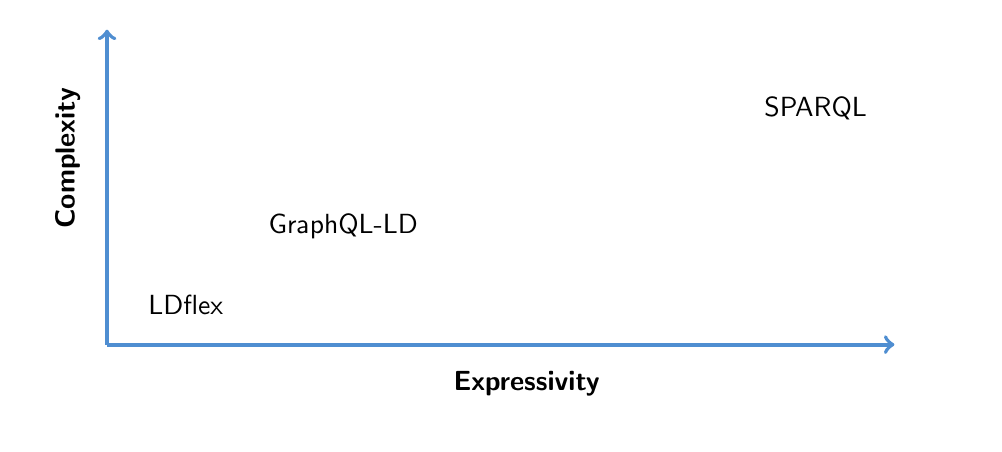
\begin{tikzpicture}[
    font={\Large\itshape},
    base/.style={font={\bfseries},inner sep=10pt,align=right,rectangle},
    txt/.style={font={},inner sep=7pt,align=center}
]

    \draw[->,line width=0.5mm,color=colorline](0, 0) -- (10, 0);
    \draw[->,line width=0.5mm,color=colorline](0, 0) -- (0, 4);
    
    \node[base,text width=10em] at (4.5, -0.5) {Expressivity};
    \node[base,text width=10em,rotate=90] at (-0.5, 1.5) {Complexity};

    \node[txt,text width=10em] at (1, 0.5) {LDflex};
    \node[txt,text width=10em] at (3, 1.5) {GraphQL-LD};
    \node[txt,text width=10em] at (9, 3) {SPARQL};

\end{tikzpicture}
\end{document}
